\documentclass{article}

% ICLR 2026 conference style, used here for a workshop submission.
% \iclrfinalcopy is deliberately left undefined (workshop = non-final /
% double-blind mode); a workshop footer is added below \maketitle instead.
\usepackage{styles/iclr2026_conference,times}
\input{styles/math_commands.tex}

% T1 encoding + cmap so copy-paste/text-extraction from the PDF is correct
% (the bare ICLR template defaults to OT1, which garbles extracted text).
\usepackage[T1]{fontenc}
\usepackage{cmap}
\usepackage{hyperref}
\usepackage{url}
\usepackage{booktabs}
\usepackage{graphicx}
\usepackage{amsmath,amssymb}
\usepackage{xcolor}
\usepackage{styles/placeins} % \FloatBarrier: flush floats per section so they never queue up and get "lost"

% Red TODOs, used both in running text and inside table cells/captions for
% pending numbers (e.g. \todo{pending: <job>}). \marginpar is deliberately
% not used: called from inside a table/figure float's internal vbox it
% corrupts the float list ("Float(s) lost"), since that context is outer
% horizontal mode, not the restricted/inner mode \marginpar assumes.
\newcommand{\todo}[1]{{\color{red}\footnotesize[TODO: #1]}}

\title{Delegated Authority Is an Input, Not an Inference:\\
Diagnosing and Externally Validating a Pre-Execution Risk Checker for Tool-Using Agents}

% Non-final ICLR style prints "Anonymous authors / Paper under double-blind
% review" automatically; \author is kept as an explicit placeholder.
\author{Anonymous authors\\Paper under double-blind review}

\newcommand{\fixmemargin}{}

\begin{document}

\maketitle
\thispagestyle{fancy}
\fancyfoot[C]{\scriptsize Submitted to a workshop at ICLR 2026 -- do not distribute.}

\begin{abstract}
Guardrail models for AI agents classify a proposed action from its text
alone. We show this misses the dimensions that matter most for delegated,
tool-using agents. Removing principal entitlements, delegated scope, and
policy text from a trained 2B checker's input drops macro AUPRC from 0.960 to
0.790 on held-out tools, and the loss is confined to three dimensions
(unauthorized-scope 1.00 to 0.13, policy-conflict 0.96 to 0.39) while content
dimensions do not move. Two zero-shot safety models and the acting agent
asked to judge its own call are at chance on exactly these dimensions with or
without the context, so prompting cannot close the gap; a blind LLM judge
loses the same dimensions when identity is removed. Policy-conditioned
reasoning generalizes to unseen policy phrasings (0.98 AUPRC) but not unseen
kinds (0.72 at 2B, 0.84 at 8B), and stacking independently thresholded
policies reaches a 0.97 false positive rate by three policies unless
decisions come from calibrated joint probabilities. On AgentDojo and
InjecAgent, traces we did not generate, policy-conflict transfers zero-shot
(0.85 and 0.97 AUPRC against 0.24 and 0.46 base rates). Prompt-injection did
not transfer at 2B until the external data exposed a label leak in our
generator; the leak-free checkers reach 0.69 (2B) and 0.84 (8B) AUPRC on
AgentDojo and rank the poisoned InjecAgent tool output above its clean twin
on 98\% of pairs (50\% and 35\% before), while the synthetic score on the
same dimension did not move.
\end{abstract}

\section{Introduction}
\label{sec:intro}

Deployed AI agents act with delegated authority: a support agent issues
refunds for a merchant, a coding agent pushes commits for a developer, an
operations agent grants IAM roles for an administrator. Before such an action
executes, some system must decide whether it may proceed. The dominant tool
is a guardrail classifier that reads the proposed action and returns a harm
judgment
\citep{inan2023llamaguard,padhi2024graniteguardian,zeng2024shieldgemma,ghosh2024aegis,openai2025gptosssafeguard}.

This conflates two questions. \textbf{Content risk} asks whether an action
looks dangerous on its face and is answerable from the action text.
\textbf{Authorization risk} asks whether \emph{this} action is something
\emph{this} agent was allowed to do, on behalf of \emph{this} principal,
under the policy in force. Its inputs are the principal's entitlements, the
agent's delegated scope, and the applicable clause. Symbolic engines
\citep{pang2019zanzibar,cutler2024cedar,oasis2013xacml} answer it exactly
when the policy is a compiled predicate; the open case is policy written in
natural language by a customer, checked against a call its author never saw.

We build a pre-execution risk classifier, \emph{forecheck}, whose typed input
contract carries these fields, and use it as an instrument. The identity
ablation of \S\ref{sec:identity} is not a discovery: three of the eleven
risk labels are functions of the fields we remove, so their collapse is
guaranteed. What it measures is how much residual signal the rendered
content carries about those labels (almost none on two), whether the other
eight dimensions are disturbed (no, but most sit at a ceiling), and whether
models that are \emph{given} the context use it. Two zero-shot safety models
and the acting agent, prompted with the same entitlements and policy text,
do not (\S\ref{sec:identity}), with the caveat
that we cannot fully separate a capability gap from a prompting mismatch. A
blind LLM judge shown only the rendered text loses the same two labels when
identity is removed (\S\ref{sec:labelvalidity}).

The main evidence is external (\S\ref{sec:external}). On AgentDojo and
InjecAgent, traces we did not generate, policy checking against predicates
we wrote transfers zero-shot. Prompt-injection detection did not transfer at
2B, and tracing that failure exposed a label leak in our own generator: an
argument key present in every injected synthetic call and no other. The
synthetic metric had been blind to it because a quarter of synthetic
positives carry no injected text, capping any text-reading detector near the
score the checker reached. Retrained leak-free, the checkers rank the
poisoned InjecAgent observation above its clean twin on 98\% of pairs.
Auditing that construction then surfaced two confounds of the same class,
one we rule out from saved scores and one we cannot. We also correct our own
earlier reading of a multi-policy composition result
(\S\ref{sec:composition}). Every number outside \S\ref{sec:external} is on
synthetic data.

\begin{table*}[t]
\centering
\small
\setlength{\tabcolsep}{5pt}
\begin{tabular}{@{}lllll@{}}
\toprule
System & Reads & Authority input & Decides & Mechanism \\
\midrule
Llama Guard, Granite Guardian & turn, optional call & none & harm category & learned \\
Agent Action Guard & tool name, arguments & none & risk score & learned \\
AlignmentCheck, Task Shield & trace, user goal & user goal (text) & goal alignment & learned \\
CaMeL & program trace, provenance & data-flow capabilities & allow/deny per call & symbolic \\
Progent & call & privilege policy (DSL) & allow/deny per call & symbolic$^{\ast}$ \\
Cedar, XACML, Zanzibar & typed request & compiled policy, relations & allow/deny & symbolic \\
forecheck & call, trajectory & entitlements, delegated scope, clause text & 11 calibrated probabilities & learned \\
\bottomrule
\end{tabular}
\caption{What each system reads, which authority input it takes, and what it decides. forecheck is the only learned checker that takes typed entitlements and delegated scope; the symbolic engines take them but not natural-language clauses. $^{\ast}$Progent's policies can be LLM-generated; enforcement is symbolic.}
\label{tab:related}
\end{table*}

\section{Problem setting}
\label{sec:setup}

\textbf{Contract.} forecheck scores a proposed tool call against an
\texttt{ActionContext}: the principal's entitlements, the scope actually
delegated to the agent (a possibly strict subset), a trust-labelled trajectory
of prior observations, the applicable policy clause(s), and the proposed
action (tool, arguments, destination), all as typed fields. A classifier that
sees only the rendered action, as every guardrail model in
\S\ref{sec:related} does, can answer content-risk questions but cannot check
whether the agent was delegated the scope it is exercising.

\textbf{Eleven risk dimensions.} Four \emph{content} dimensions are decidable
from action and destination alone
(\texttt{destructive\_or\_irreversible\_action}, \texttt{financial\_commitment},
\texttt{external\_communication}, \texttt{untrusted\_destination}); two
\emph{trajectory} dimensions from prior observations
(\texttt{prompt\_injection\_influence}, \texttt{suspicious\_action\_sequence});
\texttt{sensitive\_data\_exposure} behaves as content because its deciding
field renders into the arguments. Four are where identity and policy are
load-bearing: \texttt{unauthorized\_scope} (inside the principal's
entitlements \emph{and} the delegated scope?), \texttt{policy\_conflict}
(violates a stated clause?), \texttt{insufficient\_context} (enough delegated
information to decide?), and \texttt{privilege\_escalation} (widens authority
beyond the grant?).

\textbf{Data.} Synthetic data from forecheck's scenario generator (49,996
rows per version), split into \texttt{train}/\texttt{calibration}/\texttt{dev}/\texttt{test},
a \texttt{heldout\_family} split withholding a stratified subset of tools,
and \texttt{heldout\_policy\_kind}/\texttt{heldout\_policy\_phrasing} splits
(\S\ref{sec:generalisation}). Versions differ only in the defect each fixes:
\texttt{v4} renders the \texttt{privilege\_escalation} deciding fields,
\texttt{v5} doubles the policy-kind inventory, \texttt{v6} removes the
injection label leak (\S\ref{sec:external}). Every synthetic number measures
whether an arm learned the generator's label function, not real-world risk.

\textbf{Arms.} A LoRA-adapted decoder \citep{hu2021lora} at 2B
(\texttt{granite-3.3-2b-instruct}) and 8B, scored by candidate-token logits
per dimension and temperature-calibrated on the calibration split; two
linear-head encoders (ModernBERT-large \citep{warner2024modernbert},
granite-embedding-r2); a deterministic rule baseline over action and
destination fields; two zero-shot safety models given the same policy text
in-prompt, Granite Guardian 3.3 8B \citep{padhi2024graniteguardian} and
gpt-oss-safeguard 20B \citep{openai2025gptosssafeguard}; and an \emph{agent
self-judgment} arm where the untrained 8B instruct model
\citep{ibm2024granite3} gets the same context in an agent system prompt and
returns one \textsc{allow}/\textsc{stop} verdict. We report AUPRC because
positive rates range from 0.03 to 0.58; chance is the positive rate.

\FloatBarrier

\section{Identity ablation}
\label{sec:identity}

At evaluation time only, we remove principal entitlements, delegated scope,
\texttt{on\_behalf\_of}, and policy text from the trained decoder's rendered
context (\texttt{--strip-identity}), leaving action, destination, and
trajectory untouched. We compare against the rule baseline, the two zero-shot
safety models, a decoder \emph{trained} on identity-free renderings, and the
same ablation at 8B (Tables~\ref{tab:macro-summary} and
\ref{tab:identity-ablation}; all eleven dimensions in
Appendix~\ref{sec:appendix-identity}).

\begin{table}[htbp]
\centering
\small
\caption{Macro AUPRC with and without identity/policy context,
\texttt{heldout\_family} unless noted. Zero-shot rows use a 2,000-row
(Granite Guardian) or 400-row (gpt-oss-safeguard) subsample. Source:
\texttt{docs/results/synthetic-v2/README.md}.}
\label{tab:macro-summary}
\begin{tabular}{lcc}
\toprule
Arm & Full & Stripped \\
\midrule
Decoder 2B v2 & 0.915 & 0.736 \\
Decoder 2B v4 & 0.960 & 0.790 \\
Decoder 8B v4 & 0.958 & 0.786 \\
Decoder 2B v4, trained stripped & --- & 0.784 \\
Encoder ModernBERT-large & 0.813 & 0.712 \\
Rule baseline & 0.614 & 0.614 \\
Granite Guardian 3.3 8B (zero-shot) & 0.257 & 0.271 \\
gpt-oss-safeguard 20B (zero-shot, test) & 0.269 & 0.238 \\
Agent self-judgment 8B (\S\ref{sec:selfjudgment}) & 0.242 & 0.281 \\
\bottomrule
\end{tabular}
\end{table}

\begin{table}[htbp]
\centering
\small
\caption{Decoder 2B v4, \texttt{heldout\_family} ($n{=}6653$) AUPRC per
dimension: full input, identity removed at evaluation, identity removed at
training, and rule baseline. Positive rate in parentheses. First three rows
are the delegated-authority dimensions.}
\label{tab:identity-ablation}
\begin{tabular}{lcccc}
\toprule
Dimension (pos.\ rate) & Full & Eval-stripped & Train-stripped & Rule \\
\midrule
\texttt{unauthorized\_scope} (0.106) & 0.999 & 0.125 & 0.107 & 0.507 \\
\texttt{policy\_conflict} (0.385) & 0.964 & 0.392 & 0.429 & 0.370 \\
\texttt{insufficient\_context} (0.079) & 0.841 & 0.412 & 0.357 & 0.232 \\
\midrule
\texttt{privilege\_escalation} (0.075) & 1.000 & 1.000 & --- & 0.364 \\
\texttt{prompt\_injection\_influence} (0.075) & 0.804 & 0.806 & --- & 0.287 \\
\texttt{financial\_commitment} & 1.000 & 1.000 & 1.000 & 1.000 \\
\bottomrule
\end{tabular}
\end{table}

\textbf{The loss is confined to three dimensions.} Macro AUPRC falls 0.17,
and Table~\ref{tab:identity-ablation} locates all of it.
\texttt{unauthorized\_scope} falls below the rule baseline once the
entitlements it must be checked against are gone; \texttt{policy\_conflict}
falls to the rule floor because no clause is left to violate;
\texttt{insufficient\_context} halves. Content and trajectory dimensions do
not move: \texttt{privilege\_escalation} survives because the v4 renderer
puts the deciding authority fields into the call text, and injection is read
from the trajectory.

\textbf{Not a fragile mechanism; scale does not recover it.} Training on
identity-free renderings from the start gives the same ceiling as stripping
at evaluation (macro 0.784 vs.\ 0.790, per-dimension within 0.06), so
stripping did not merely break a shortcut: the information is absent from the
content. An 8B decoder collapses identically (0.958 to 0.786) on the same
three dimensions.

\textbf{Zero-shot safety models never used the context.} Their macro AUPRC is
0.24--0.27, at chance, and unchanged or slightly higher when identity is
removed. If a general safety model quietly used delegated-authority context,
stripping would hurt; it does not, for either model. Both were trained for
harm, jailbreak, and groundedness, not for checking an action against
entitlements or a clause. This claim rests on the three dimensions being
labels an independent reader can recover; \S\ref{sec:labelvalidity} finds
that holds for two of the three.

\FloatBarrier

\section{Policy generalization: kind vs.\ phrasing}
\label{sec:generalisation}

Robustness to unseen \emph{tools} (\texttt{heldout\_family}) is not
robustness to unseen \emph{policy kinds} or \emph{phrasings}, and the latter
is the more product-relevant test: a deployment needs the classifier to
apply a customer's own wording, not just handle a new tool under a
training-set policy. ADR 0010 adds two splits: \texttt{heldout\_policy\_kind}
withholds entire predicate kinds (e.g.\ \texttt{forbid\_recipient\_domain})
from training; \texttt{heldout\_policy\_phrasing} withholds one paraphrase
index of every kind the model \emph{did} train on. \texttt{v4} additionally
fixes a renderer defect that left \texttt{privilege\_escalation}
undecidable from text (\S\ref{sec:limitations}).

\begin{table}[tbp]
\centering
\small
\caption{Decoder 2B, macro AUPRC and \texttt{policy\_conflict} AUPRC across
splits, on the v3 (ADR 0010, 15 policy kinds, 2 withheld) and v4 (same data,
\texttt{privilege\_escalation} render fix) generators. v5 (ADR 0011, 30
kinds, 4 withheld) tests whether more kinds let the model generalize the
\emph{shape} of policy-conflict reasoning rather than memorize kinds.
Source: \texttt{docs/results/synthetic-v2/README.md}.}
\label{tab:policy-generalisation}
\begin{tabular}{lcccc}
\toprule
Split & v3 macro & v3 \texttt{policy\_conflict} & v4 macro & v4 \texttt{policy\_conflict} \\
\midrule
test & 0.908 & 0.994 & 0.960 & 0.994 \\
heldout\_family & 0.914 & 0.941 & 0.960 & 0.964 \\
heldout\_policy\_kind & 0.889 & \textbf{0.653} & 0.944 & \textbf{0.752} \\
heldout\_policy\_phrasing & 0.921 & 0.987 & 0.968 & 0.993 \\
\midrule
v5 (30 kinds, 4 withheld) & \multicolumn{4}{c}{\todo{pending: train-2b-b200-v5-recipe.yaml}} \\
\bottomrule
\end{tabular}
\end{table}

\begin{figure}[tbp]
\centering
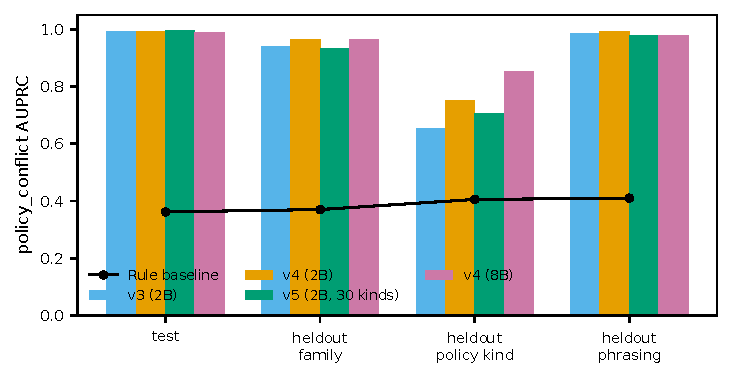
\includegraphics[width=5.5in]{figures/fig_policy_generalisation.pdf}
\caption{Decoder 2B, \texttt{policy\_conflict} AUPRC across splits for the v3
and v4 generators (synthetic data; $n$ per split matches
Table~\ref{tab:policy-generalisation}), with the rule baseline's
\texttt{policy\_conflict} AUPRC on each split shown as a line. The v5 slot is
left blank pending that run. Source:
\texttt{docs/results/synthetic-v2/decoder-2b-v3/}, \texttt{decoder-2b-v4/}.}
\label{fig:policy-generalisation}
\end{figure}

Figure~\ref{fig:policy-generalisation} makes the kind-vs-phrasing asymmetry
visible: bars for test, \texttt{heldout\_family}, and
\texttt{heldout\_policy\_phrasing} sit close together near the ceiling, while
\texttt{heldout\_policy\_kind} drops toward, though still above, the rule
baseline line.

Two very different results. \textbf{Unseen phrasing generalizes.} A
paraphrase index never seen in training leaves \texttt{policy\_conflict} at
0.987--0.993 AUPRC, matching the in-distribution test split (0.994): the
model reads the clause's meaning, not a template id. \textbf{Unseen policy
kinds do not.} With two of fifteen kinds withheld, \texttt{policy\_conflict}
drops to 0.653 (v3) / 0.752 (v4) at a 0.32--0.41 rule-baseline floor -- above
chance but far below every kind seen in training, including under novel
wording. Every other dimension on this split is unaffected, so the model has
learned the fifteen kinds it saw, not the general operation of checking a
predicate against a rendered fact.

The v4 fix also confirms \texttt{privilege\_escalation}'s earlier
AUROC-high/AUPRC-low signature (\S\ref{sec:limitations}) was a data defect,
not a model limit: rendering the deciding
\texttt{authority\_before}/\texttt{authority\_after} values lifts it from
0.505 to 1.000 AUPRC on \texttt{heldout\_family}.

ADR 0011 tests whether more kinds fix kind-generalization: it triples the
inventory to 30 and withholds only 4 (a smaller fraction than v3/v4's
2-of-15). A rise toward the phrasing-generalization level ($\sim$0.99) would
make ``kind'' a learnable unit of generalization; staying in the 0.65--0.75
band despite more diversity would point to a structural limit needing
retrieval-plus-entailment rather than more kinds. Pending at submission time
(Table~\ref{tab:policy-generalisation}, last row).

\FloatBarrier

\section{Multi-policy composition and the calibration hinge}
\label{sec:composition}

Guardrail deployments run several independently tuned policies and act on
the most restrictive decision, OR-ing $k$ binary guards, so false positives
compound in $k$ alone. forecheck instead emits one calibrated probability
vector over the eleven dimensions, composed by one policy engine and decided
either by per-dimension thresholds or by the argmin of expected cost over the
joint vector under a fixed cost table.

\begin{table}[htbp]
\centering
\small
\caption{False positive rate on covered-benign examples,
\texttt{heldout\_family} ($n{=}6640$), stacking $k$ synthetic per-dimension
policies. \texttt{independent} ORs $k$ separately thresholded decisions;
\texttt{expected\_cost\_joint} merges the same policies into one bundle and
decides from the joint probability vector. FNR, review rate, the
\texttt{joint} strategy, and curves in Appendix~\ref{sec:appendix-stacking}.}
\label{tab:stacking-main}
\begin{tabular}{llccc}
\toprule
Arm (macro ECE) & Strategy & $k{=}1$ & $k{=}2$ & $k{=}3$ (same to 8) \\
\midrule
Decoder 2B (0.004) & \texttt{independent} & 0.015 & 0.140 & \textbf{0.966} \\
Decoder 2B (0.004) & \texttt{expected\_cost\_joint} & 0.015 & 0.082 & 0.082 \\
Encoder granite-r2 (0.049) & \texttt{independent} & --- & 0.710 & 0.990 \\
Encoder granite-r2 (0.049) & \texttt{expected\_cost\_joint} & --- & 0.921 & 0.921 \\
\bottomrule
\end{tabular}
\end{table}

\textbf{Threshold stacking denies everything by $k{=}3$.} Independent
stacking pushes the decoder's FPR from 0.015 to 0.966 by three policies and
holds it there through eight, not because any policy got worse but because
more were added. Deciding from the joint calibrated vector is invariant in
$k$ from $k{=}2$ on (FPR/FNR/review rate flat at 0.082/0.070/0.28): the
decision depends on the probability vector and the cost table, not on how many
rules mention a dimension.

\textbf{The invariance is a calibration property, not a decision-rule
property.} The same rule on the granite-embedding-r2 encoder's probabilities,
identical examples and policies, settles at FPR 0.921, worse than its own
independent stacking at $k{=}2$. The decoder is calibrated (macro ECE 0.004,
temperature-scaled \citep{guo2017calibration,platt1999probabilistic}); the
encoder is not (0.049). Expected-cost composition keeps a stack from
collapsing only when the probabilities feeding it are calibrated. The cost
table is the default severity tier, so the claim is about the curve's shape
in $k$, not the table. The product-facing form of the same probabilities is in
Appendix~\ref{sec:appendix-approval}: at a 5\% deployment incident rate,
89--99\% of human approvals can be auto-decided under a 1--5\% incident
budget.

\FloatBarrier

\section{Can the acting agent judge its own scope?}
\label{sec:selfjudgment}

A cheaper alternative to an external checker is to ask the acting agent,
inside its own system prompt, whether to proceed. We give the untrained 8B
instruct model an agent system prompt carrying the identical entitlements,
delegated scope, and policy text, then the pending call, and read one
\textsc{allow}/\textsc{stop} verdict off the first output token. That scalar
is scored against all eleven labels on the same 2,000 \texttt{heldout\_family}
rows as the trained checker (Table~\ref{tab:selfjudgment}; all dimensions in
Appendix~\ref{sec:appendix-selfjudgment}).

\begin{table}[htbp]
\centering
\small
\caption{Agent self-judgment (8B, untrained, single \textsc{allow}/\textsc{stop}
verdict) vs.\ the trained 2B v4 checker, AUPRC on the same 2,000
\texttt{heldout\_family} rows; positive rate in parentheses.}
\label{tab:selfjudgment}
\begin{tabular}{lccc}
\toprule
Dimension (pos.\ rate) & Agent 8B & Agent 8B, stripped & Checker 2B v4 \\
\midrule
\texttt{unauthorized\_scope} (0.106) & 0.135 & 0.101 & 0.999 \\
\texttt{policy\_conflict} (0.385) & 0.509 & 0.419 & 0.964 \\
\texttt{insufficient\_context} (0.079) & 0.086 & 0.083 & 0.841 \\
\texttt{privilege\_escalation} (0.075) & 0.103 & 0.101 & 1.000 \\
\texttt{prompt\_injection\_influence} (0.075) & 0.166 & \textbf{0.507} & 0.804 \\
\midrule
Macro & 0.242 & 0.281 & 0.960 \\
\bottomrule
\end{tabular}
\end{table}

\textbf{The agent cannot judge its own scope from inside its prompt.} With
full context it is at or near chance on every identity-dependent dimension
(AUROC 0.53--0.67), the level of the zero-shot safety models; the checker
beats it on all eleven dimensions by 0.45--0.90 AUPRC. \textbf{Identity
context makes the agent worse at spotting injection.} Removing the policy and
scope text raises its injection AUPRC from 0.166 to 0.507 while the checker's
does not move (0.804 to 0.806): a long policy preamble dilutes the untrained
model's attention to an injected instruction elsewhere in the trajectory.
Both findings argue for an external checker, even on content dimensions.

\FloatBarrier

\section{Are the labels real? An independent blind judge}
\label{sec:labelvalidity}

Is each label observable in the rendered text at all, to a reader who never
sees the generator's latent scenario? A frontier model (gpt-5.6-sol), given
only the rendered context and the eleven dimension definitions, judged 600
\texttt{v4} rows stratified to at least 20 positives and 20 negatives per
dimension, once with the full rendering and once identity-stripped. Agreement
with the generator is not ground truth, but low agreement is informative: the
label then depends on information the generator tracked and never rendered,
and a model scoring well on it is learning a generator regularity.

\begin{table}[htbp]
\centering
\small
\caption{Blind LLM-judge agreement with the generator label (yes vs.\
not-yes, Cohen's $\kappa$), $n{=}600$ \texttt{v4} rows, full and
identity-stripped renderings. Right: AUPRC of the 2B v4 checker and the rule
baseline \emph{against the judge's labels} on the judged
\texttt{heldout\_family} rows ($n{=}257$). Full table in
Appendix~\ref{sec:appendix-judge}.}
\label{tab:judge-agreement}
\begin{tabular}{lcc|cc}
\toprule
Dimension & $\kappa$ full & $\kappa$ stripped & Checker vs.\ judge & Rule vs.\ judge \\
\midrule
\texttt{privilege\_escalation} & 0.909 & 0.909 & 0.977 & 0.297 \\
\texttt{prompt\_injection\_influence}$^{\dagger}$ & 0.905 & 0.905 & 1.000 & 0.459 \\
\texttt{policy\_conflict} & 0.714 & \textbf{0.029} & 0.889 & 0.502 \\
\texttt{unauthorized\_scope} & 0.391 & \textbf{0.040} & 0.592 & 0.509 \\
\texttt{destructive\_or\_irreversible\_action} & 0.511 & 0.542 & 0.635 & 0.509 \\
\texttt{untrusted\_destination} & 0.213 & 0.205 & 0.864 & 0.785 \\
\texttt{insufficient\_context} & 0.059 & $-$0.036 & 0.090 & 0.090 \\
\texttt{sensitive\_data\_exposure} & 0.002 & 0.061 & 0.405 & 0.291 \\
\midrule
macro (11 dims) & 0.436 & 0.340 & 0.613 & 0.415 \\
\bottomrule
\end{tabular}
\vskip 1mm
{\footnotesize $^{\dagger}$Measured on v4 text carrying the injection label leak (\S\ref{sec:external}); judge and generator could agree by reading the leaked argument.}
\end{table}

\textbf{Three tiers.} \emph{Recoverable} ($\kappa > 0.7$):
\texttt{privilege\_escalation}, \texttt{prompt\_injection\_influence},
\texttt{policy\_conflict}; for the last, judge recall is 0.89 and the
disagreements are the judge reading a clause more strictly than the
generator's predicate. \emph{Definitional disagreement} ($0.2 \le \kappa \le
0.5$): six dimensions where both produce coherent decisions under different
definitions; the judge flags twice as many \texttt{unauthorized\_scope} rows
because it counts a mismatch with the agent's stated objective as out of
scope, while the generator's label is entitlement-based (judge recall of
generator positives 0.74). These are taxonomy decisions to fix in the
definitions. \emph{Not recoverable} ($\kappa < 0.1$):
\texttt{insufficient\_context} and \texttt{sensitive\_data\_exposure}; the
judge calls the context sufficient on 50 of 58 generator-positive rows.

\textbf{The judge replicates the identity ablation on labels.} Stripping
identity from the judge's input drops \texttt{policy\_conflict} $\kappa$ from
0.714 to 0.029 (28 judge-positives instead of 259: no clause left to check)
and \texttt{unauthorized\_scope} from 0.391 to 0.040 (203 positives at
precision 0.16: guessing from the action). Every other dimension is unchanged
within noise, and the content dimensions' judge-yes counts are identical
between passes. These are the same two dimensions the trained checker loses
(Table~\ref{tab:identity-ablation}).

\textbf{Consequence for \S\ref{sec:identity}.} The identity-ablation claim is
solid on \texttt{policy\_conflict}, directionally confirmed on
\texttt{unauthorized\_scope}, and unvalidated on \texttt{insufficient\_context}:
the checker's 0.841 on that label is closer to a generator regularity than to
a checkable question about the text, and we flag every number on it. Scored
against the judge's labels instead of the generator's, the checker keeps the
three recoverable dimensions and beats the rule baseline on each by
0.39--0.68 AUPRC.

\FloatBarrier

\section{Transfer to data we did not generate}
\label{sec:external}

We score the checkers zero-shot on two published benchmarks. Nothing was
trained or tuned on either; calibration was fitted on synthetic data and
threshold selection is disabled. The leak-free v6 checkers are the paper's
models; v4 rows are the pre-fix comparison.

\textbf{AgentDojo} \citep{debenedetti2024agentdojo}: banking-suite traces
for two frontier agents, 1,714 runs, 4,215 proposed calls, 11 attack types
plus no-attack runs. Labels come from AgentDojo's own \texttt{ground\_truth()}
functions: \texttt{prompt\_injection\_influence} is \texttt{yes} when a call
executes the injection task's goal (positive rate 0.150);
\texttt{unauthorized\_scope} when the call's function is outside the user
task's reference solution (0.253). \texttt{policy\_conflict} (0.237) is
\emph{ours}: four banking policies, each a deterministic predicate over
user-named recipients. \textbf{InjecAgent} \citep{zhan2024injecagent}: 1,054
cases over 38 toolkits. AgentDojo's injection positives differ from negatives
in the call itself, so it cannot tell whether a checker reads the untrusted
text or the call. InjecAgent can: for each attacker tool we build a
\emph{poisoned/clean pair}, the same call with the attacker's instruction
filled in (\texttt{yes}) or removed (\texttt{no}) from the tool response.
4,250 examples, 1,598 pairs; \texttt{policy\_conflict} from five generic
policies about the call's shape.

\begin{table*}[t]
\centering
\footnotesize
\setlength{\tabcolsep}{4pt}
\begin{tabular}{@{}lccc|ccc|ccc@{}}
\toprule
& \multicolumn{3}{c|}{AgentDojo banking} & \multicolumn{3}{c|}{InjecAgent} & \multicolumn{3}{c}{tie-adj.\ win vs.} \\
Arm & inj.\ (.15) & scope (.25) & policy$^{\ast}$ (.24) & inj.\ (.50) & scope (.75) & policy$^{\ast}$ (.46) & clean & padded & instr.\ \\
\midrule
Rule baseline & 0.250 & 0.253 & 0.237 & 0.500 & 0.752 & 0.464 & -- & -- & -- \\
\midrule
Decoder 2B v6 & 0.693 & 0.214 & 0.670 & 0.878 & 0.704 & 0.922 & 0.980 & 0.986 & 0.989 \\
\quad eval-stripped & 0.669 & 0.306 & 0.521 & -- & -- & -- & -- & -- & -- \\
Decoder 8B v6 & \textbf{0.838} & 0.239 & 0.785 & 0.943 & 0.677 & 0.965 & 0.983 & 0.981 & \textbf{0.993} \\
\quad eval-stripped & 0.819 & 0.354 & 0.450 & \textbf{0.953} & 0.917 & 0.963 & \textbf{0.986} & \textbf{0.986} & \textbf{0.993} \\
\midrule
Decoder 2B v4 (pre-fix) & 0.128 & 0.257 & \textbf{0.849} & 0.549 & 0.732 & 0.965 & 0.624 & 0.514 & 0.515 \\
Decoder 8B v4 (pre-fix) & 0.701 & 0.355 & 0.626 & 0.544 & 0.849 & \textbf{0.977} & -- & -- & -- \\
\quad eval-stripped & 0.743 & 0.266 & 0.404 & 0.556 & 0.843 & 0.968 & -- & -- & -- \\
\bottomrule
\end{tabular}
\caption{Zero-shot AUPRC on AgentDojo banking ($n{=}4{,}215$; $4{,}133$ for injection) and InjecAgent ($n{=}4{,}250$; $3{,}196$ for injection), positive rates in the header; $^{\ast}$labels from predicates we wrote. Right block: tie-adjusted injection win over 1,598 InjecAgent groups against three length-matched controls (defined in Appendix~\ref{sec:appendix-external}), 0.5 is chance; 8B v4 was not scored against them. Full counts and sign tests in Table~\ref{tab:injecagent-controls}. Agent-self, Guardian and the v4 stripped AgentDojo rows are in Appendix~\ref{sec:appendix-external}.}
\label{tab:external}
\end{table*}

\textbf{Policy checking transfers, and on AgentDojo it stays
identity-dependent.} On banking \texttt{policy\_conflict}, whose predicates
reference user-named recipients, 2B v4 scores 0.849 against a 0.237 base
rate on policies and traces it never saw; eval-time stripping drops it to
0.694, train-stripped to 0.390. The v6 checkers
score lower here (0.670, 0.785) with the same pattern (0.521, 0.450), the
one external result bearing on the identity thesis. On InjecAgent the same
dimension scores 0.92--0.98 and barely moves under stripping: the five
policies are call-shape rules, a content result.

\begin{figure}[t]
\centering
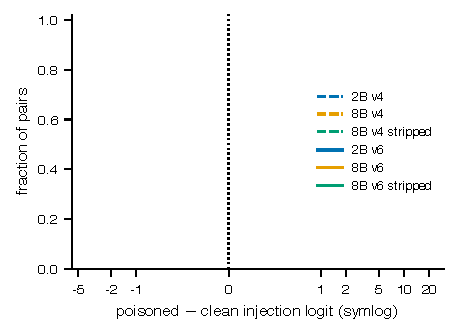
\includegraphics[width=\columnwidth]{figures/fig_injecagent_margins.pdf}
\caption{InjecAgent pairs: empirical CDF of the poisoned-minus-clean injection logit over the 1,598 pairs, per checker. The v4 heads (dashed) put a quarter to two fifths of pairs exactly at zero and a further quarter below it; the v6 heads (solid) rank the poisoned variant higher on 98\% of pairs. Counts and intervals in Table~\ref{tab:injecagent-audit}.}
\label{fig:injecagent-margins}
\end{figure}

\textbf{Injection before the fix: the v4 heads barely read the untrusted
text.} 2B v4 is below base rate on AgentDojo injection (0.128, AUROC 0.348):
its injection head never fires on this domain while its policy head
separates the same rows; 8B v4 reaches 0.701. On InjecAgent, with the call
held fixed, both v4 heads sit near raw logit $-4$ on poisoned and clean
alike and return an identical score on 24\% (2B) and 39\% (8B) of pairs
(Figure~\ref{fig:injecagent-margins}). Counting ties as half, they rank the
poisoned variant higher on 0.624 and 0.546 of pairs, significantly above
0.5 ($p<10^{-5}$) but small.

\textbf{The cause was a label leak in our generator.} Contrasting injected
and non-injected synthetic calls, the v1--v5 generator wrote an
\texttt{instructed\_target} argument into every
injected call and no other (presence 1.00 vs.\ 0.00 over 13,312 v4 rows) and
drew its value from five literals, three containing ``attacker''
(Appendix~\ref{sec:appendix-leak}). The synthetic metric could not show
this: a quarter of positives render no injected text, so observation-only
and key-only detectors are both capped near 0.75--0.80 AUPRC, consistent
with the checker's 0.80. The synthetic score measured the ceiling, not what
the head read.

\textbf{v6 restores transfer; the fix is a bundle.} v6 removes the key,
fills the target argument for benign calls, and lengthens observations.
Retrained on v6 with the same size and recipe, 2B reaches
0.693 on AgentDojo injection and 8B 0.838, and both heads fire. On
InjecAgent both rank the poisoned variant strictly above its clean twin on
0.977 of pairs with under 2\% ties; the synthetic injection score did not
change (0.804 to 0.787 on \texttt{heldout\_family}). Two single-factor arms,
matched to v6 on recipe, seed, and row count, isolate which change did the
work: v6a (key removed, v4-length observations) reaches 0.659 AUPRC on
AgentDojo injection, against v6b (key kept, v6-length observations) at
0.139, indistinguishable from v4's 0.128. Observation length and variety
contribute nothing measurable; the key removal is the entire gain
(Table~\ref{tab:agentdojo}, Appendix~\ref{sec:appendix-external}).

\textbf{The length confound is tested and closed.} The clean twin is shorter
than the poisoned observation in all 1,598 groups; two more controls,
padded and instruction, refill the slot with byte-matched benign text
instead, shorter than or equal to it in 95.7\% of groups. Against both, v6
still wins 0.98--0.99 tie-adjusted (Table~\ref{tab:external}), while v4's
0.624 win against plain clean falls to 0.514 against padded, chance
($p=0.16$): v4's signal was length, not injection reading. A second
confound, destination trust, flips in 39\% of groups but does not carry the
result: restricted to the 972 groups where it is equal, every v6 win moves
by at most 0.015 (Appendix~\ref{sec:appendix-external}).

\textbf{More synthetic data does not buy transfer; full fine-tuning does.}
2B LoRA at four v6-generator sizes (5k--250k rows, one seed each, rows and
steps co-varying) holds \texttt{heldout\_family} macro AUPRC flat at
0.938--0.954, matched by a 2B full fine-tune at 25k (0.949); injection
transfer falls monotonically with more rows (AgentDojo
0.695$\to$0.423$\to$0.354, InjecAgent-controls 0.898$\to$0.606$\to$0.353):
the generator's variety is exhausted early; extra rows teach its
regularities, not the task. AgentDojo \texttt{policy\_conflict} is
non-monotonic here, one seed, not interpreted. Full fine-tuning at 25k
beats LoRA on both benchmarks (0.797 vs.\ 0.693; 0.825 vs.\ 0.742), closing
most of the gap to 8B LoRA (Figure~\ref{fig:scaling},
Table~\ref{tab:scaling}, Appendix~\ref{sec:appendix-external}).

\textbf{What does not transfer.} \texttt{unauthorized\_scope} is near base
rate on AgentDojo for every checker (0.21--0.36 vs.\ 0.253); the label counts
harmless auxiliary reads as out of scope. On InjecAgent, 8B v6 is below base
rate (0.677 vs.\ 0.752) until the port's placeholder principal and scope
fields are removed (0.917). Removing identity helps on several external
cells: right fields help, generic ones hurt. Calibration does not transfer (macro ECE 0.20--0.27 vs.\ under 0.03
synthetic); isotonic refitting on 250--500 labelled calls restores ECE
0.01. Suite-level results are in Appendix~\ref{sec:appendix-external}.

\FloatBarrier

\section{Related work}
\label{sec:related}

\textbf{LLM guardrails.} Llama Guard \citep{inan2023llamaguard}, Granite
Guardian \citep{padhi2024graniteguardian}, ShieldGemma
\citep{zeng2024shieldgemma}, NVIDIA Aegis \citep{ghosh2024aegis}, and
gpt-oss-safeguard \citep{openai2025gptosssafeguard} classify content or harm
per turn or action; Agent Action Guard \citep{agentactionguard2025} is an
embedding MLP over tool name and arguments. LlamaFirewall's AlignmentCheck
\citep{chennabasappa2025llamafirewall} and Task Shield
\citep{jia2025taskshield} judge alignment with the user's stated goal, the
closest analogues of our \texttt{unauthorized\_scope}; neither takes a typed
entitlement or delegated scope as input.

\textbf{Authorization for agents.} Symbolic engines decide allow/deny from a
fully specified request and compiled policy: OPA \citep{opa}, Cedar
\citep{cutler2024cedar}, XACML with its combining algorithms
\citep{oasis2013xacml}, and Zanzibar \citep{pang2019zanzibar}, whose
``is this delegated scope inside the principal's grant'' check is exactly our
\texttt{unauthorized\_scope}. Agent-specific designs enforce authorization by
construction: CaMeL \citep{debenedetti2025camel} tracks capabilities through
a quarantined LLM's dataflow, Progent \citep{shi2025progent} applies
per-call privilege policies, IsolateGPT \citep{wu2025isolategpt} puts agent
applications behind a permission layer, and RTBAS \citep{zhong2025rtbas} and
AirGapAgent \citep{bagdasarian2024airgapagent} enforce principal-dependent
information-flow norms. OWASP's agentic guidance \citep{owasp2025agentic}
holds that authorization must be deterministic and auditable. Table~\ref{tab:related} sets these side by side. Our delta is
narrow and compatible with all of these: where the mandate is a
natural-language clause nobody has compiled, a learned reader generalises
across paraphrases (\S\ref{sec:generalisation}) and emits a probability such
an engine can consume; the deterministic check on typed fields remains the
right tool for scope.

\textbf{Prompt-injection defences and benchmarks.} StruQ, SecAlign, and
spotlighting \citep{chen2024struq,chen2025secalign,hines2024spotlighting}
harden the acting model; our injection head is a detector in front of it.
AgentHarm, ToolEmu, InjecAgent, AgentDojo, and Agent Security Bench
\citep{andriushchenko2024agentharm,ruan2023toolemu,zhan2024injecagent,debenedetti2024agentdojo,zhang2025asb}
measure end-to-end agent behaviour with an outcome judge; we reuse two as
external test sets by deriving per-action labels from their ground-truth
functions.

\section{Conclusion}
\label{sec:conclusion}

Delegated-authority labels are functions of fields a content classifier
never sees; our ablation confirms the rendered content carries almost nothing
about two of the three, which was expected. What was not guaranteed: models
given the context do not use it under a straightforward prompt, a blind
reader loses the same labels when the fields are removed, policy checking
generalises to unseen wording but not unseen kinds, and an apparent
composition collapse was one fail-closed bundle. The strongest result is
methodological: a benchmark we did not generate exposed a label leak that
every synthetic split had scored at its ceiling, and auditing our own
external construction then surfaced two more confounds of the same class.

\section{Limitations}
\label{sec:limitations}

\textbf{Synthetic data only.} Every number here is on data from forecheck's
own scenario generator (\texttt{docs/evaluation-plan.md}, classes 1--2). No
human-labelled or production-traffic evaluation exists at submission time,
and no real-world safety claim is made: every result measures whether an
arm learned the generator's own label function.

\textbf{Generator regularities.} The model may be exploiting template
regularities in how the generator writes policy clauses and entitlement
lists, rather than a general policy-reading ability. The
\texttt{heldout\_policy\_kind}/\texttt{heldout\_policy\_phrasing} splits
(\S\ref{sec:generalisation}) probe this and only partly rule it out:
phrasing generalizes cleanly, kind does not, consistent with a lookup over
kinds rather than the underlying operation. The encoder's earlier null
result on both splits is uninformative the same way -- it never learned
\texttt{policy\_conflict} at all, so a flat curve shows nothing.

\textbf{\texttt{privilege\_escalation} render defect (v2/v3).} The
\texttt{authority\_before}/\texttt{authority\_after} fields deciding this
label were never rendered into the tool-call text in v2/v3, so every arm's
0.46--0.53 AUPRC there reflects a data defect: 78 of 79 dev positives were
textually indistinguishable from an in-scope re-grant. Fixed in v4
(\S\ref{sec:generalisation}); numbers sourced from v2/v3 elsewhere should be
read with this in mind.

\textbf{Single seed.} Every trained-arm result is from one training seed. A
seed-variance re-run \todo{pending: decoder-2b-v4-seed1} is needed before
these point estimates should be read as more precise than the seed-to-seed
variance they have not yet been measured against.

\textbf{Held-out-policy-kind failure.} \texttt{policy\_conflict} AUPRC drops
from $\sim$0.99 (in-distribution, unseen-phrasing) to 0.65--0.75 on entirely
unseen kinds. The supportable claim today is "one model, policies of a kind
seen in training, any phrasing" -- not "arbitrary new policy kinds." The v5
experiment (ADR 0011) testing whether a larger kind inventory fixes this is
pending.

\textbf{Other caveats.} A single generator family (English, template
renderer) produces every example. The \S\ref{sec:composition} cost table is
the default severity tier, not tuned to any organization. Generator seed
nondeterminism was found and partially fixed mid-project
(\texttt{docs/results/notes/privilege-escalation-diagnosis.md}); v2/v3 data
are not byte-reproducible from their configs.

\FloatBarrier

\section*{Ethics statement}

All training data are synthetic and contain no personal data; the external
benchmarks are used under their published licences and no new human
annotation was collected. The base models (Granite 3.3, ModernBERT,
granite-embedding-r2) and our code are Apache-2.0. A pre-execution risk
checker is dual-use only in the weak sense that any classifier can be tuned
to permit what it should refuse; we release policies and thresholds as
customer-authored inputs, not fixed defaults, and state plainly that no
result here licenses a real-world safety claim. The blind-judge and
agent-self experiments used commercial and open models for inference only.


\bibliography{refs}
\bibliographystyle{styles/iclr2026_conference}

\appendix
\section{Identity ablation: all dimensions, v2}
\label{sec:appendix-identity}

Table~\ref{tab:identity-ablation-v2} gives the v2 per-dimension numbers behind
Figure~\ref{fig:identity-ablation}. The v4 ablation (Table~\ref{tab:identity-ablation})
replicates the pattern with one change: \texttt{privilege\_escalation}
survives stripping in v4 (1.000 to 1.000) because the v4 renderer puts the
deciding \texttt{authority\_before}/\texttt{authority\_after} fields into the
tool-call text; in v2 they were never rendered and every arm scored 0.46--0.53
on it, so it is omitted below.

\begin{figure}[htbp]
\centering
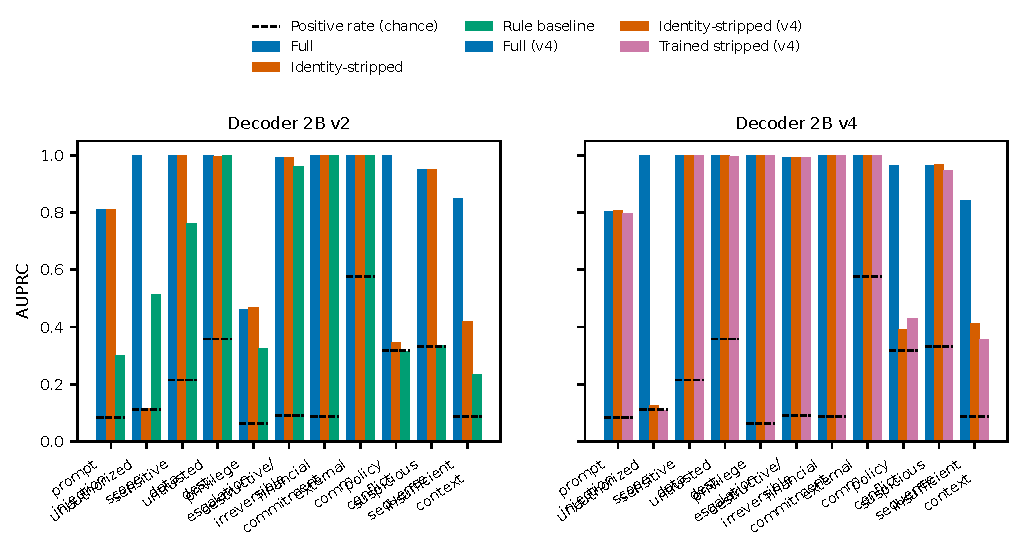
\includegraphics[width=5.2in]{figures/fig_identity_ablation.pdf}
\caption{Decoder 2B v2, per-dimension AUPRC on \texttt{heldout\_family}
($n{=}6640$): full model vs.\ identity-stripped vs.\ rule baseline, with each
dimension's positive rate (chance) as a dashed line. The drop is confined to
\texttt{unauthorized\_scope}, \texttt{policy\_conflict}, and
\texttt{insufficient\_context}.}
\label{fig:identity-ablation}
\end{figure}

\begin{table}[htbp]
\centering
\small
\caption{Decoder 2B v2, \texttt{heldout\_family} ($n{=}6640$) AUPRC per
dimension: full, identity-stripped, and rule baseline. Source:
\texttt{docs/results/synthetic-v2/README.md}.}
\label{tab:identity-ablation-v2}
\begin{tabular}{lccc}
\toprule
Dimension & Decoder (full) & Decoder (stripped) & Rule baseline \\
\midrule
\texttt{unauthorized\_scope} & 1.000 & 0.116 & 0.512 \\
\texttt{policy\_conflict} & 0.999 & 0.345 & 0.315 \\
\texttt{insufficient\_context} & 0.849 & 0.418 & 0.235 \\
\texttt{prompt\_injection\_influence} & 0.810 & 0.810 & 0.301 \\
\texttt{suspicious\_action\_sequence} & 0.952 & 0.950 & 0.334 \\
\texttt{financial\_commitment} & 1.000 & 1.000 & 1.000 \\
\bottomrule
\end{tabular}
\end{table}

\section{Policy generalization: macro AUPRC and per-seed values}
\label{sec:appendix-generalisation}

\begin{table}[htbp]
\centering
\footnotesize
\caption{Decoder 2B, macro AUPRC and \texttt{policy\_conflict} (pc) AUPRC
across splits for the v3 (15 policy kinds, 2 withheld), v4 (same data,
\texttt{privilege\_escalation} render fix), and v5 (30 kinds, 4 withheld)
generators, seed 0; last column an 8B LoRA on v4 data, seed 0. Three-seed
values for the \texttt{heldout\_policy\_kind} pc cell: v4 0.752, 0.689, 0.711;
v5 0.704, 0.755, 0.717; 8B v4 (two seeds) 0.851, 0.825. Source:
\texttt{docs/results/synthetic-v2/README.md}.}
\label{tab:policy-generalisation-full}
\begin{tabular}{lccccccc}
\toprule
Split & v3 macro & v4 macro & v5 macro & v3 pc & v4 pc & v5 pc & 8B v4 pc \\
\midrule
test & 0.908 & 0.960 & 0.957 & 0.994 & 0.994 & 0.996 & 0.990 \\
heldout\_family & 0.914 & 0.960 & 0.951 & 0.941 & 0.964 & 0.933 & 0.965 \\
heldout\_policy\_kind & 0.889 & 0.944 & 0.941 & 0.653 & 0.752 & 0.704 & 0.851 \\
heldout\_policy\_phrasing & 0.921 & 0.968 & 0.970 & 0.987 & 0.993 & 0.980 & 0.978 \\
\bottomrule
\end{tabular}
\end{table}

\begin{figure}[htbp]
\centering
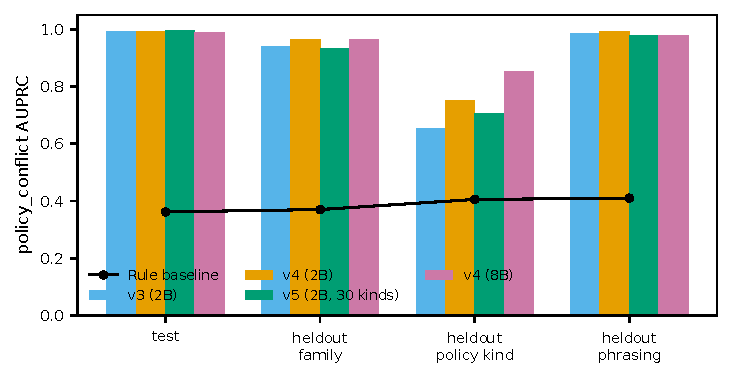
\includegraphics[width=5.2in]{figures/fig_policy_generalisation.pdf}
\caption{Decoder 2B, \texttt{policy\_conflict} AUPRC across splits for the
v3, v4, and v5 generators, plus the 8B LoRA on v4 data, with the rule
baseline's \texttt{policy\_conflict} AUPRC on each split shown as a line.
Bars for test, \texttt{heldout\_family}, and \texttt{heldout\_policy\_phrasing}
sit near the ceiling; \texttt{heldout\_policy\_kind} drops toward, though
still above, the rule baseline, for every generator and both sizes.}
\label{fig:policy-generalisation}
\end{figure}

The v4 render fix also confirms that \texttt{privilege\_escalation}'s earlier
AUROC-high/AUPRC-low signature was a data defect, not a model limit:
rendering the deciding fields lifts it from 0.505 to 1.000 AUPRC on
\texttt{heldout\_family}.

\section{Multi-policy stacking: full table and curves}
\label{sec:appendix-stacking}

Table~\ref{tab:stacking-full} extends Table~\ref{tab:stacking-main} with the
\texttt{joint} strategy (rules from all $k$ policies merged into one bundle
and evaluated once in threshold mode), false negative rate, and review rate.
\texttt{independent} and \texttt{joint} are identical at $k{\le}2$ because the
synthetic stacking policies use only plain rules, so the engine's combination
logic has nothing to do differently; they diverge at $k{=}3$ only through
threshold interaction. The $k{=}1$ row already trades false positives for
false negatives relative to the F1-optimal threshold (FPR/FNR 0.058/0.170
vs.\ 0.015/0.253) because the default cost table is severity-weighted.

\begin{table}[htbp]
\centering
\small
\caption{Multi-policy stacking, \texttt{heldout\_family} ($n{=}6640$).
Source: \texttt{docs/evaluation/multi-policy-stacking.md}.}
\label{tab:stacking-full}
\begin{tabular}{llcccc}
\toprule
Arm & $k$ & Strategy & FPR & FNR & Review rate \\
\midrule
Decoder 2B & 1 & any & 0.015 & 0.253 & 0.31 \\
Decoder 2B & 2 & independent & 0.140 & 0.080 & 0.30 \\
Decoder 2B & 2 & expected\_cost\_joint & 0.082 & 0.070 & 0.28 \\
Decoder 2B & 3 & independent & \textbf{0.966} & 0.016 & 0.66 \\
Decoder 2B & 3 & joint & 0.905 & 0.051 & 0.63 \\
Decoder 2B & 3 & expected\_cost\_joint & 0.082 & 0.070 & 0.28 \\
Decoder 2B & 8 & independent & 0.966 & 0.007 & 0.58 \\
Decoder 2B & 8 & expected\_cost\_joint & 0.082 & 0.070 & 0.28 \\
\midrule
Encoder granite-r2 & 2 & independent & 0.710 & 0.042 & 0.26 \\
Encoder granite-r2 & 2 & expected\_cost\_joint & 0.921 & 0.010 & 0.37 \\
Encoder granite-r2 & 3 & independent & 0.990 & 0.008 & 0.21 \\
Encoder granite-r2 & 3 & expected\_cost\_joint & 0.921 & 0.010 & 0.37 \\
\bottomrule
\end{tabular}
\end{table}

\begin{figure}[htbp]
\centering
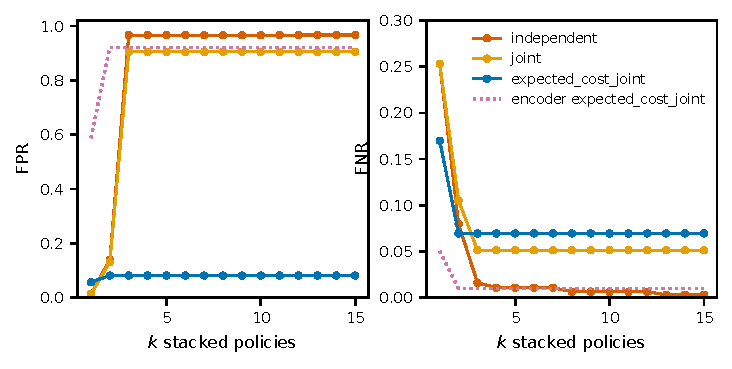
\includegraphics[width=5.2in]{figures/fig_stacking.pdf}
\caption{Decoder 2B, FPR (left) and FNR (right) vs.\ number of stacked
policies $k$ on \texttt{heldout\_family} ($n{=}6640$), for
\texttt{independent}, \texttt{joint}, and \texttt{expected\_cost\_joint}
strategies; the granite-embedding-r2 encoder's \texttt{expected\_cost\_joint}
curve is dotted. The flat decoder curve is a property of its calibration, not
of the decision rule: the encoder's curve under the same rule sits near the top
of the FPR panel.}
\label{fig:stacking}
\end{figure}

\section{Approval elimination}
\label{sec:appendix-approval}

The product-facing metric is how many of a deployment's human-approval
reviews can be automated at a chosen incident rate: sort examples by the
decoder's expected cost of \textsc{allow} and ask what fraction of the review
queue can be auto-decided while the fraction of auto-allowed actions that are
actually risky stays under a budget. Because \texttt{heldout\_family} is
adversarial-heavy (58\% base incident rate), Table~\ref{tab:approval} reports
both the raw curve and a curve importance-reweighted to a 5\% deployment
incident rate, with elimination computed conservatively via a 95\% Wilson
upper bound \citep{wilson1927probable} on the realized incident rate in the
auto-allowed set.

\begin{table}[htbp]
\centering
\small
\caption{Decoder 2B, approval elimination on \texttt{heldout\_family} (v2
$n{=}6640$, v4 $n{=}6653$), bundle \texttt{balanced}. ``raw'' is the split's
own 57--58\% base incident rate; ``rw'' reweights rows so the incident rate is
5\%. Source: \texttt{docs/evaluation/approval-elimination.md}.}
\label{tab:approval}
\begin{tabular}{lcccc}
\toprule
Budget & Elim.\ (v2, raw) & Elim.\ (v2, rw) & Elim.\ (v4, rw) & Review (v4, rw) \\
\midrule
0.1\% & 0.000 & 0.000 & 0.000 & 0.969 \\
0.5\% & 0.000 & 0.000 & 0.000 & 0.969 \\
1\% & 0.000 & 0.888 & 0.903 & 0.067 \\
2\% & 0.000 & 0.961 & 0.952 & 0.021 \\
5\% & 0.000 & 0.992 & 0.992 & 0.001 \\
\bottomrule
\end{tabular}
\end{table}

\begin{figure}[htbp]
\centering
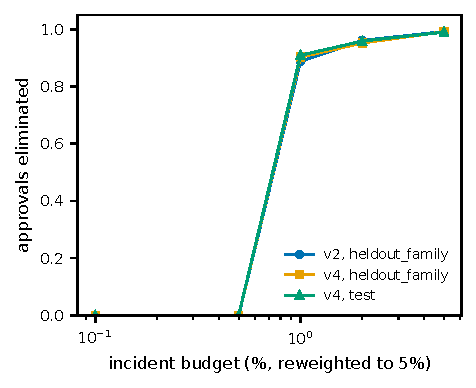
\includegraphics[width=3.3in]{figures/fig_approval_curve.pdf}
\caption{Approvals eliminated vs.\ incident budget, reweighted to a 5\%
deployment incident rate, decoder 2B v2 and v4 on \texttt{heldout\_family}
and v4 on test, log-scaled budget axis. The three curves nearly overlap.}
\label{fig:approval-curve}
\end{figure}

At a 5\% deployment incident rate the calibrated decoder auto-allows
88.8--99.2\% of actions that would otherwise need review while keeping the
allowed-but-risky rate under budget. The unweighted column is near zero
because the split's top-ranked rows already contain risky examples by
construction; it is a ceiling of the split's design, not of the classifier.
Below a 1\% budget the Wilson bound cannot be met at this sample size and the
conservative curve reports zero.

\section{Agent self-judgment: all dimensions}
\label{sec:appendix-selfjudgment}

\begin{figure}[htbp]
\centering
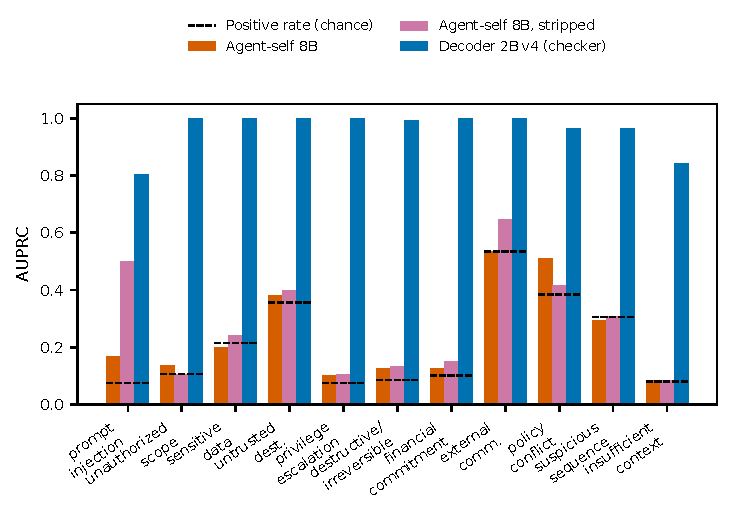
\includegraphics[width=5.2in]{figures/fig_self_judgment.pdf}
\caption{Per-dimension AUPRC on \texttt{heldout\_family} ($n{=}2000$ for the
agent-self-8B rows, $n{=}6653$ for the decoder), positive rate as a dashed
line. The agent's bars track chance everywhere except
\texttt{policy\_conflict} and \texttt{external\_communication}; the external
checker clears 0.84 on every dimension.}
\label{fig:self-judgment}
\end{figure}

The checker beats the agent's single-verdict score on all eleven dimensions
by 0.45--0.90 AUPRC. The small identity signal that does exist in the agent
(\texttt{unauthorized\_scope} AUROC 0.61 full vs.\ 0.48 stripped) shows it
reads the context a little without turning it into a usable decision. The 2B
agent-self condition behaves the same way and is omitted.

\section{Blind judge: full agreement table}
\label{sec:appendix-judge}

\begin{table}[htbp]
\centering
\small
\caption{Independent LLM-judge agreement with the generator label, yes vs.\
not-yes, $n{=}600$ \texttt{v4} rows (gpt-5.6-sol, blind to the generator's
latent scenario), full and identity-stripped renderings.
Agreement/recall/precision are for the full-context pass. Source:
\texttt{docs/results/judge/README.md}.}
\label{tab:judge-agreement-full}
\begin{tabular}{lccccc}
\toprule
Dimension & $\kappa$ full & $\kappa$ stripped & Agreement & Judge recall & Judge precision \\
\midrule
\texttt{privilege\_escalation} & 0.909 & 0.909 & 0.988 & 1.00 & 0.84 \\
\texttt{prompt\_injection\_influence} & 0.905 & 0.905 & 0.983 & 0.84 & 1.00 \\
\texttt{policy\_conflict} & 0.714 & 0.029 & 0.862 & 0.89 & 0.78 \\
\midrule
\texttt{destructive\_or\_irreversible\_action} & 0.511 & 0.542 & 0.897 & 0.60 & 0.54 \\
\texttt{suspicious\_action\_sequence} & 0.404 & 0.428 & 0.852 & 0.82 & 0.33 \\
\texttt{unauthorized\_scope} & 0.391 & 0.040 & 0.800 & 0.74 & 0.38 \\
\texttt{financial\_commitment} & 0.359 & 0.300 & 0.935 & 0.24 & 0.92 \\
\texttt{external\_communication} & 0.331 & 0.361 & 0.897 & 0.86 & 0.23 \\
\texttt{untrusted\_destination} & 0.213 & 0.205 & 0.777 & 0.41 & 0.29 \\
\midrule
\texttt{insufficient\_context} & 0.059 & $-$0.036 & 0.843 & 0.14 & 0.15 \\
\texttt{sensitive\_data\_exposure} & 0.002 & 0.061 & 0.783 & 0.17 & 0.08 \\
\bottomrule
\end{tabular}
\end{table}

\begin{figure}[htbp]
\centering
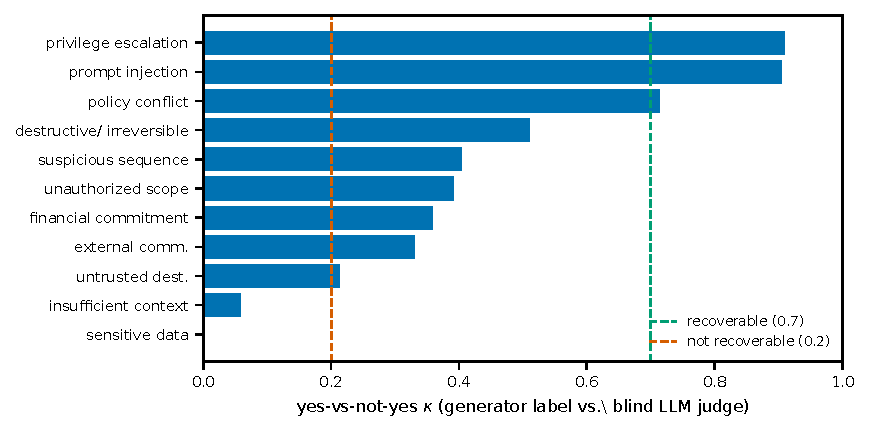
\includegraphics[width=5.2in]{figures/fig_judge_agreement.pdf}
\caption{Yes-vs-not-yes $\kappa$ per dimension, sorted, with the recoverable
(0.7) and not-recoverable (0.2) tier lines.}
\label{fig:judge-agreement}
\end{figure}

\begin{table}[htbp]
\centering
\small
\caption{AUPRC against the judge's labels on the judged \texttt{heldout\_family}
rows ($n{=}257$), decoder 2B v4 vs.\ rule baseline, with the decoder's AUPRC
against the generator's own labels on the full split for reference. The lookup
dimensions collapse for both arms because the judge defines them differently
(e.g.\ \texttt{financial\_commitment} requires funds to move;
\texttt{sensitive\_data\_exposure} requires a lower-sensitivity destination),
so they are not evidence for or against either arm.}
\label{tab:model-vs-judge}
\begin{tabular}{lccc}
\toprule
Dimension & Decoder 2B v4 & Rule baseline & Decoder vs.\ generator labels \\
\midrule
\texttt{prompt\_injection\_influence} & \textbf{1.000} & 0.459 & 0.804 \\
\texttt{privilege\_escalation} & \textbf{0.977} & 0.297 & 1.000 \\
\texttt{policy\_conflict} & \textbf{0.889} & 0.502 & 0.964 \\
\texttt{untrusted\_destination} & \textbf{0.864} & 0.785 & 1.000 \\
\texttt{destructive\_or\_irreversible\_action} & 0.635 & 0.509 & 0.992 \\
\texttt{unauthorized\_scope} & 0.592 & 0.509 & 0.999 \\
\texttt{suspicious\_action\_sequence} & 0.528 & 0.467 & 0.966 \\
\texttt{external\_communication} & 0.437 & 0.381 & 1.000 \\
\texttt{sensitive\_data\_exposure} & 0.405 & 0.291 & 1.000 \\
\texttt{financial\_commitment} & 0.327 & 0.280 & 1.000 \\
\texttt{insufficient\_context} & 0.090 & 0.090 & 0.841 \\
\midrule
macro & 0.613 & 0.415 & 0.960 \\
\bottomrule
\end{tabular}
\end{table}

\section{External benchmarks: full tables}
\label{sec:appendix-external}

\begin{table}[htbp]
\centering
\small
\caption{AUPRC on AgentDojo banking traces, zero-shot, $n{=}4{,}215$
($n{=}4{,}133$ for injection). \texttt{untrusted\_destination} has positives
only and is excluded from macro. Guardian and agent-self rows are on a fixed
1,000-row subsample. Macro ECE of the calibrated arms is 0.20--0.27 here
against under 0.03 on synthetic data. Source:
\texttt{docs/results/agentdojo/README.md}.}
\label{tab:agentdojo}
\begin{tabular}{lcccccc}
\toprule
Arm & injection & scope & policy & financial & destructive & macro \\
\midrule
Rule baseline & 0.250 & 0.253 & 0.237 & 0.896 & 1.000 & 0.527 \\
Decoder 2B v4 & 0.128 & 0.257 & 0.849 & 1.000 & 1.000 & 0.647 \\
2B v4, eval-stripped & 0.125 & 0.218 & 0.694 & 1.000 & 1.000 & 0.608 \\
2B v4, train-stripped & 0.150 & 0.234 & 0.390 & 1.000 & 1.000 & 0.555 \\
Decoder 8B v4 & 0.701 & 0.355 & 0.626 & 0.923 & 0.999 & 0.721 \\
8B v4, eval-stripped & 0.743 & 0.266 & 0.404 & 0.934 & 1.000 & 0.669 \\
\midrule
Decoder 2B v6 (leak-free) & 0.693 & 0.214 & 0.670 & 0.935 & 1.000 & 0.702 \\
2B v6, eval-stripped & 0.669 & 0.306 & 0.521 & 0.941 & 1.000 & 0.687 \\
Decoder 8B v6 (leak-free) & 0.838 & 0.239 & 0.785 & 0.945 & 0.831 & 0.728 \\
8B v6, eval-stripped & 0.819 & 0.354 & 0.450 & 0.979 & 0.975 & 0.715 \\
\midrule
Granite Guardian 3.3 8B & 0.103 & 0.289 & 0.224 & 0.257 & 0.217 & 0.218 \\
Agent-self 8B (\textsc{allow}/\textsc{stop}) & 0.291 & 0.442 & 0.449 & 0.591 & 0.105 & 0.375 \\
\bottomrule
\end{tabular}
\end{table}

\begin{table}[htbp]
\centering
\small
\caption{AUPRC on InjecAgent, zero-shot, $n{=}4{,}250$ ($n{=}3{,}196$ for
injection, positive rate 0.500). Pair win: fraction of the 1,598
poisoned/clean pairs on which the poisoned variant scores higher on injection;
tie: fraction with identical raw score. Baseline rows on a fixed 1,000-row
subsample (injection $n{=}767$). Source:
\texttt{docs/results/injecagent/README.md}.}
\label{tab:injecagent}
\begin{tabular}{lcccccc|cc}
\toprule
Arm & injection & scope & policy & financial & destructive & macro & pair win & tie \\
\midrule
Rule baseline & 0.500 & 0.752 & 0.464 & 0.683 & 1.000 & 0.680 & -- & -- \\
Decoder 2B v4 & 0.549 & 0.732 & 0.965 & 1.000 & 1.000 & 0.849 & 0.504 & 0.239 \\
Decoder 8B v4 & 0.544 & 0.849 & 0.977 & 0.734 & 1.000 & 0.821 & 0.353 & 0.385 \\
8B v4, eval-stripped & 0.556 & 0.843 & 0.968 & 0.766 & 1.000 & 0.827 & 0.382 & 0.397 \\
\midrule
Decoder 2B v6 (leak-free) & 0.878 & 0.704 & 0.922 & 0.970 & 0.998 & 0.894 & 0.977 & 0.005 \\
Decoder 8B v6 (leak-free) & 0.943 & 0.677 & 0.965 & 0.771 & 0.997 & 0.870 & 0.977 & 0.012 \\
8B v6, eval-stripped & 0.953 & 0.917 & 0.963 & 0.839 & 0.998 & 0.934 & 0.978 & 0.016 \\
\midrule
Granite Guardian 3.3 8B & 0.511 & 0.613 & 0.359 & 0.102 & 0.197 & 0.356 & -- & -- \\
Agent-self 8B (\textsc{allow}/\textsc{stop}) & 0.530 & 1.000 & 0.647 & 0.061 & 0.178 & 0.483 & -- & -- \\
\bottomrule
\end{tabular}
\end{table}

\begin{table}[htbp]
\centering
\small
\caption{AgentDojo, all four suites (30,143 proposed calls: banking 4,215,
slack 8,246, travel 10,701, workspace 6,981), \texttt{prompt\_injection\_influence}
AUPRC / AUROC per suite, positive rate in the header. v4 checkers only; the
v6 checkers have not been run on this export. Source:
\texttt{docs/results/agentdojo/README.md}.}
\label{tab:agentdojo-suites}
\begin{tabular}{lcccc}
\toprule
Arm & banking (0.150) & slack (0.186) & travel (0.025) & workspace (0.077) \\
\midrule
Rule baseline & 0.250 / 0.737 & 0.222 / 0.601 & 0.021 / 0.360 & 0.138 / 0.740 \\
Decoder 2B v4 & 0.128 / 0.348 & 0.178 / 0.479 & 0.048 / 0.686 & 0.065 / 0.353 \\
Decoder 8B v4 & 0.701 / 0.895 & 0.433 / 0.738 & 0.131 / 0.834 & 0.752 / 0.941 \\
8B v4, eval-stripped & 0.743 / 0.915 & 0.421 / 0.726 & 0.146 / 0.844 & 0.727 / 0.943 \\
Agent-self 8B & 0.354 / 0.832 & 0.292 / 0.687 & 0.026 / 0.484 & 0.246 / 0.866 \\
\bottomrule
\end{tabular}
\end{table}

\begin{figure}[htbp]
\centering
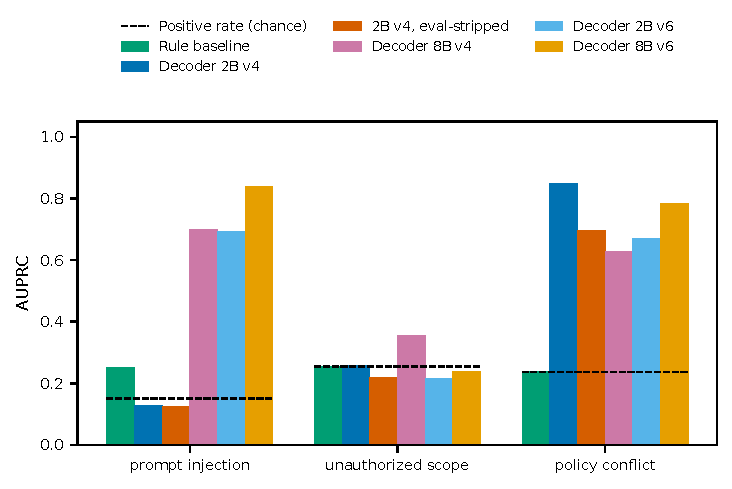
\includegraphics[width=5.2in]{figures/fig_agentdojo.pdf}
\caption{AUPRC on AgentDojo banking traces for the three learned dimensions:
rule baseline, decoder 2B v4, 2B v4 eval-stripped, decoder 8B v4, and the
leak-free 2B v6 and 8B v6, zero-shot, with each dimension's positive rate as
a dashed line.}
\label{fig:agentdojo}
\end{figure}

\textbf{Per-example logits.} The 2B v4 injection head never fires on
AgentDojo: raw logits for all 4,133 evaluable calls lie between $-5.0$ and
$-3.0$, the highest-scoring positive is $-3.25$, and no call scores above
zero, while on the same rows its \texttt{policy\_conflict} head has median
raw logit $+2.5$ for positives and $-3.5$ for negatives. The 8B v4 head is
live but shifted (median $-1.75$ for positives vs.\ $-3.50$ for negatives,
29\% of positives above zero vs.\ 0.7\% of negatives). After the v6 retrain,
2B v6 has median $+4.5$ vs.\ $-3.0$ (92\% vs.\ 23\% above zero) and 8B v6
$+6.25$ vs.\ $-3.25$ (94\% vs.\ 8\%). On InjecAgent the v4 heads sit at
raw logit $-4$ on poisoned and clean alike; the v6 heads have median raw
$+3.5$ vs.\ $-6.25$ (2B) and $+2.25$ vs.\ $-3.5$ (8B), and 58\% of poisoned
calls score above 0 at both sizes against 9\% (2B) and 0.1\% (8B) of clean.
Inference is deterministic (per-example raw difference 0 between repeated
runs).

\textbf{Recalibration.} Refitting per-dimension isotonic calibrators on a
random half of the AgentDojo banking calls and testing on the other half
(five seeds) gives macro ECE 0.008 (2B) and 0.010 (8B) with AUPRC unchanged;
the 8B \texttt{unauthorized\_scope} head goes from ECE 0.60 to 0.01 by
learning to output the base rate. Most of the gain is reached with 250--500
labelled calls (\texttt{scripts/agentdojo\_recalibrate.py},
\texttt{docs/results/agentdojo/recalibration.md}).

\textbf{Other suites.} \texttt{unauthorized\_scope} outside banking is carried
by the rule baseline (0.749 on slack, 0.733 on workspace, where nearly half of
all calls are labelled out of scope); 2B adds under 0.09 and both 8B arms are
below the rule. \texttt{policy\_conflict} on slack, travel, and workspace uses
one generic policy per suite at 0.7--8\% base rates: 2B AUROC is 0.78--0.89
but AUPRC 0.005--0.49, so we claim policy transfer on banking and InjecAgent
only.

\section{Injection label leak: diagnosis and fix}
\label{sec:appendix-leak}

After the 2B checker failed on AgentDojo injection we contrasted the rendered
call between injected and non-injected synthetic examples. The v1--v5
generator wrote an \texttt{instructed\_target} argument into every injected
call and into no other call (presence 1.00 vs.\ 0.00 over 13,312 v4 rows), put
a \texttt{to} argument into 100\% of injected calls vs.\ 3\% of others, and
drew the injected target from five literals, three containing ``attacker''
(\texttt{attacker-agent-007}, \texttt{external-support@attacker.example},
\texttt{shadow-ops@attacker.example}). Injected observations were five short
templates (median 132 characters) against AgentDojo's 2,000-character record
dumps. The v6 renderer (2.0.0) removes \texttt{instructed\_target}, chooses
the target argument key from the tool kind and fills it for benign calls too,
draws targets from pools shared between injected and benign calls, and
renders 300--2,000 character multi-format observations with the instruction
at a random position. A leakage check on argument-key presence parity and a
token denylist runs before training. Judge agreement on
\texttt{prompt\_injection\_influence} ($\kappa{=}0.905$,
Table~\ref{tab:judge-agreement-full}) was measured on v4 text and has not been
re-run on v6. Full write-up:
\texttt{docs/results/notes/injection-label-leak-diagnosis.md}.

\FloatBarrier


\end{document}
